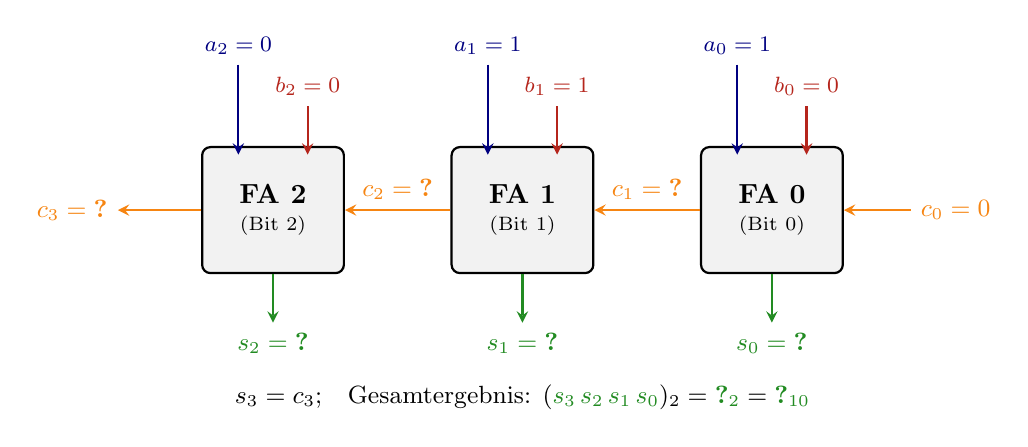
\begin{tikzpicture}[
    scale=0.88, >=stealth,
    fa/.style={draw, thick, fill=gray!10, rounded corners=3pt, minimum width=1.8cm, minimum height=1.6cm, align=center}
]
    % FA Blocks
    \node[fa] (fa2) at (0, 0) {\textbf{FA 2}\\[-2pt]{\scriptsize (Bit 2)}};
    \node[fa] (fa1) at (3.6, 0) {\textbf{FA 1}\\[-2pt]{\scriptsize (Bit 1)}};
    \node[fa] (fa0) at (7.2, 0) {\textbf{FA 0}\\[-2pt]{\scriptsize (Bit 0)}};

    % Inputs from top (a_i in NavyBlue, b_i in BrickRed)
    \draw[thick, ->, NavyBlue] (-0.5, 2.1) node[above, font=\footnotesize, NavyBlue] {$a_2 = 0$} -- (-0.5, 0.8);
    \draw[thick, ->, BrickRed] (0.5, 1.5) node[above, font=\footnotesize, BrickRed] {$b_2 = 0$} -- (0.5, 0.8);

    \draw[thick, ->, NavyBlue] (3.1, 2.1) node[above, font=\footnotesize, NavyBlue] {$a_1 = 1$} -- (3.1, 0.8);
    \draw[thick, ->, BrickRed] (4.1, 1.5) node[above, font=\footnotesize, BrickRed] {$b_1 = 1$} -- (4.1, 0.8);

    \draw[thick, ->, NavyBlue] (6.7, 2.1) node[above, font=\footnotesize, NavyBlue] {$a_0 = 1$} -- (6.7, 0.8);
    \draw[thick, ->, BrickRed] (7.7, 1.5) node[above, font=\footnotesize, BrickRed] {$b_0 = 0$} -- (7.7, 0.8);

    % Carry chain in BurntOrange (right to left)
    \draw[thick, ->, BurntOrange] (9.2, 0) node[right, font=\small, BurntOrange] {$c_0 = 0$} -- (fa0.east);
    \draw[thick, ->, BurntOrange] (fa0.west) -- (fa1.east) node[midway, above, font=\small, BurntOrange] {$c_1 = \textbf{?}$};
    \draw[thick, ->, BurntOrange] (fa1.west) -- (fa2.east) node[midway, above, font=\small, BurntOrange] {$c_2 = \textbf{?}$};
    \draw[thick, ->, BurntOrange] (fa2.west) -- ++(-1.2, 0) node[left, font=\small, BurntOrange] {$c_3 = \textbf{?}$};

    % Sum outputs in ForestGreen (to bottom)
    \draw[thick, ->, ForestGreen] (fa2.south) -- ++(0, -0.7) node[below, font=\small, ForestGreen] {$s_2 = \textbf{?}$};
    \draw[thick, ->, ForestGreen] (fa1.south) -- ++(0, -0.7) node[below, font=\small, ForestGreen] {$s_1 = \textbf{?}$};
    \draw[thick, ->, ForestGreen] (fa0.south) -- ++(0, -0.7) node[below, font=\small, ForestGreen] {$s_0 = \textbf{?}$};

    % Result line (spaced well below sum outputs)
    \node[font=\small, align=center] at (3.6, -2.7) {$s_3=c_3$;\quad Gesamtergebnis: $(\textcolor{ForestGreen}{s_3 \, s_2 \, s_1 \, s_0})_2 = \textcolor{ForestGreen}{\textbf{?}_2} = \textcolor{ForestGreen}{\textbf{?}_{10}}$};
\end{tikzpicture}
